% Options for packages loaded elsewhere
\PassOptionsToPackage{unicode}{hyperref}
\PassOptionsToPackage{hyphens}{url}
%
\documentclass[
  english,
  man]{apa6}
\usepackage{amsmath,amssymb}
\usepackage{lmodern}
\usepackage{iftex}
\ifPDFTeX
  \usepackage[T1]{fontenc}
  \usepackage[utf8]{inputenc}
  \usepackage{textcomp} % provide euro and other symbols
\else % if luatex or xetex
  \usepackage{unicode-math}
  \defaultfontfeatures{Scale=MatchLowercase}
  \defaultfontfeatures[\rmfamily]{Ligatures=TeX,Scale=1}
\fi
% Use upquote if available, for straight quotes in verbatim environments
\IfFileExists{upquote.sty}{\usepackage{upquote}}{}
\IfFileExists{microtype.sty}{% use microtype if available
  \usepackage[]{microtype}
  \UseMicrotypeSet[protrusion]{basicmath} % disable protrusion for tt fonts
}{}
\makeatletter
\@ifundefined{KOMAClassName}{% if non-KOMA class
  \IfFileExists{parskip.sty}{%
    \usepackage{parskip}
  }{% else
    \setlength{\parindent}{0pt}
    \setlength{\parskip}{6pt plus 2pt minus 1pt}}
}{% if KOMA class
  \KOMAoptions{parskip=half}}
\makeatother
\usepackage{xcolor}
\IfFileExists{xurl.sty}{\usepackage{xurl}}{} % add URL line breaks if available
\IfFileExists{bookmark.sty}{\usepackage{bookmark}}{\usepackage{hyperref}}
\hypersetup{
  pdftitle={Getting a Step Ahead: Using the Regularized Horseshoe Prior to Select Cross-Loadings in Bayesian CFA},
  pdflang={en-EN},
  hidelinks,
  pdfcreator={LaTeX via pandoc}}
\urlstyle{same} % disable monospaced font for URLs
\usepackage{graphicx}
\makeatletter
\def\maxwidth{\ifdim\Gin@nat@width>\linewidth\linewidth\else\Gin@nat@width\fi}
\def\maxheight{\ifdim\Gin@nat@height>\textheight\textheight\else\Gin@nat@height\fi}
\makeatother
% Scale images if necessary, so that they will not overflow the page
% margins by default, and it is still possible to overwrite the defaults
% using explicit options in \includegraphics[width, height, ...]{}
\setkeys{Gin}{width=\maxwidth,height=\maxheight,keepaspectratio}
% Set default figure placement to htbp
\makeatletter
\def\fps@figure{htbp}
\makeatother
\setlength{\emergencystretch}{3em} % prevent overfull lines
\providecommand{\tightlist}{%
  \setlength{\itemsep}{0pt}\setlength{\parskip}{0pt}}
\setcounter{secnumdepth}{-\maxdimen} % remove section numbering
% Make \paragraph and \subparagraph free-standing
\ifx\paragraph\undefined\else
  \let\oldparagraph\paragraph
  \renewcommand{\paragraph}[1]{\oldparagraph{#1}\mbox{}}
\fi
\ifx\subparagraph\undefined\else
  \let\oldsubparagraph\subparagraph
  \renewcommand{\subparagraph}[1]{\oldsubparagraph{#1}\mbox{}}
\fi
\newlength{\cslhangindent}
\setlength{\cslhangindent}{1.5em}
\newlength{\csllabelwidth}
\setlength{\csllabelwidth}{3em}
\newlength{\cslentryspacingunit} % times entry-spacing
\setlength{\cslentryspacingunit}{\parskip}
\newenvironment{CSLReferences}[2] % #1 hanging-ident, #2 entry spacing
 {% don't indent paragraphs
  \setlength{\parindent}{0pt}
  % turn on hanging indent if param 1 is 1
  \ifodd #1
  \let\oldpar\par
  \def\par{\hangindent=\cslhangindent\oldpar}
  \fi
  % set entry spacing
  \setlength{\parskip}{#2\cslentryspacingunit}
 }%
 {}
\usepackage{calc}
\newcommand{\CSLBlock}[1]{#1\hfill\break}
\newcommand{\CSLLeftMargin}[1]{\parbox[t]{\csllabelwidth}{#1}}
\newcommand{\CSLRightInline}[1]{\parbox[t]{\linewidth - \csllabelwidth}{#1}\break}
\newcommand{\CSLIndent}[1]{\hspace{\cslhangindent}#1}
% This preamble allows to remove the redundant title page from papaja's output.pdf
\usepackage{atbegshi}% http://ctan.org/pkg/atbegshi
\AtBeginDocument{\AtBeginShipoutNext{\AtBeginShipoutDiscard}}
% Manuscript styling
\usepackage{upgreek}
\captionsetup{font=singlespacing,justification=justified}

% Table formatting
\usepackage{longtable}
\usepackage{lscape}
% \usepackage[counterclockwise]{rotating}   % Landscape page setup for large tables
\usepackage{multirow}		% Table styling
\usepackage{tabularx}		% Control Column width
\usepackage[flushleft]{threeparttable}	% Allows for three part tables with a specified notes section
\usepackage{threeparttablex}            % Lets threeparttable work with longtable

% Create new environments so endfloat can handle them
% \newenvironment{ltable}
%   {\begin{landscape}\centering\begin{threeparttable}}
%   {\end{threeparttable}\end{landscape}}
\newenvironment{lltable}{\begin{landscape}\centering\begin{ThreePartTable}}{\end{ThreePartTable}\end{landscape}}

% Enables adjusting longtable caption width to table width
% Solution found at http://golatex.de/longtable-mit-caption-so-breit-wie-die-tabelle-t15767.html
\makeatletter
\newcommand\LastLTentrywidth{1em}
\newlength\longtablewidth
\setlength{\longtablewidth}{1in}
\newcommand{\getlongtablewidth}{\begingroup \ifcsname LT@\roman{LT@tables}\endcsname \global\longtablewidth=0pt \renewcommand{\LT@entry}[2]{\global\advance\longtablewidth by ##2\relax\gdef\LastLTentrywidth{##2}}\@nameuse{LT@\roman{LT@tables}} \fi \endgroup}

% \setlength{\parindent}{0.5in}
% \setlength{\parskip}{0pt plus 0pt minus 0pt}

% \usepackage{etoolbox}
\makeatletter
\patchcmd{\HyOrg@maketitle}
  {\section{\normalfont\normalsize\abstractname}}
  {\section*{\normalfont\normalsize\abstractname}}
  {}{\typeout{Failed to patch abstract.}}
\patchcmd{\HyOrg@maketitle}
  {\section{\protect\normalfont{\@title}}}
  {\section*{\protect\normalfont{\@title}}}
  {}{\typeout{Failed to patch title.}}
\makeatother
\shorttitle{Getting a Step Ahead: Using the Regularized Horseshoe Prior to Select Cross-Loadings in Bayesian CFA}
\keywords{\newline\indent Word count: X}
\DeclareDelayedFloatFlavor{ThreePartTable}{table}
\DeclareDelayedFloatFlavor{lltable}{table}
\DeclareDelayedFloatFlavor*{longtable}{table}
\makeatletter
\renewcommand{\efloat@iwrite}[1]{\immediate\expandafter\protected@write\csname efloat@post#1\endcsname{}}
\makeatother
\usepackage{csquotes}
\ifXeTeX
  % Load polyglossia as late as possible: uses bidi with RTL langages (e.g. Hebrew, Arabic)
  \usepackage{polyglossia}
  \setmainlanguage[]{english}
\else
  \usepackage[main=english]{babel}
% get rid of language-specific shorthands (see #6817):
\let\LanguageShortHands\languageshorthands
\def\languageshorthands#1{}
\fi
\ifLuaTeX
  \usepackage{selnolig}  % disable illegal ligatures
\fi

\title{Getting a Step Ahead: Using the Regularized Horseshoe Prior to Select Cross-Loadings in Bayesian CFA}
\author{\phantom{0}}
\date{}


\affiliation{\phantom{0}}

\begin{document}
\maketitle

% move text to bottom of page
\vfill
Research Report\\
Michael Koch (6412157)\\
Methodology and Statistics for the Behavioral, Biomedical, and Social Sciences \\
Supervisor: Dr. Sara van Erp \\ 
Email: j.m.b.koch@students.uu.nl \\
Word Count: 2500 \\
Intented Journal of Publication: Structural Equation Modeling \\

% make page numbers start from second page 
\pagenumbering{arabic}
\setcounter{page}{0}
\thispagestyle{empty}
% make page numbers from second page 
\pagestyle{plain}

\clearpage

\begin{figure}
\centering
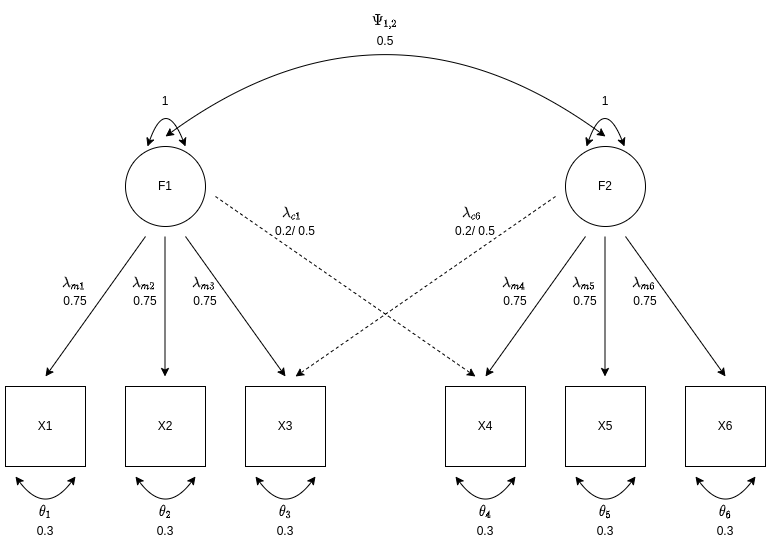
\includegraphics{~/OneDrive/ms/thesis/Rmd/figures/model.png}
\caption{Graphical Representation of the True Model.}
\end{figure}

The art of statistical modeling revolves around coming up with an appropriate simplification, a \emph{model}, of a true \emph{data-generating process}. Hereby, a fundamental trade-off between model simplicity and model complexity arises, that is mostly knownw under the term \emph{bias-variance trade-off}. Simple models with few parameters have high bias, meaning that they deviate substantially from the true data-generating process. However, these models have low variance, hence they generalize well to other datasets from the same popoulation. Moreover, simple models are easily identified (estimatable with the information available in the data) and easy to interpret. Complex models with large numbers of parameters tend to have low levels of bias, i.e.~they tend to accurately represent the data generating process. However, complex models tend to have high variance. Consquently, complex models are prone to over-fitting, i.e.~picking up patterns that are only relevant in the dataset at hand, but do not generalize well to other datasets. Moreover, complex models can be cumbersome to interpret and often a large number of observations is required to estimate them (Cox, 2006; James, Witten, Hastie, \& Tibshirani, 2021).

\hypertarget{regularization}{%
\subsection{Regularization}\label{regularization}}

A classic way of dealing with the bias-variance trade-off is \emph{regularization} (Hastie, Tibshirani, \& Wainwright, 2015). Here, during the estimation process of a model it is actively chosen to add some bias to the model to reduce its variance. This helps to ensure that the model becomes easier to interpret and more generalizable. In a frequentist context, regularization is achieved by adding a penality term to the cost function of a model. Such penality ensures that some model parameters that are deemed irrelevant, e.g.~small regression coefficients in a regression model with a large number of predictors, are shrunken to (or towards) zero. In a Bayesian context, the same is achieved by setting a so-called shrinkage-prior (Van Erp, Oberski, \& Mulder, 2019) for the parameter in question. Hereby, for every frequentist penality term a bayesian counterpart exist (Van Erp et al., 2019). For instance, the well-known ridge- (Hoerl \& Kennard, 2000) and lasso-penalization (Tibshirani, 1996) in regression correspond to setting a ridge-prior (Hsiang, 1975) and a laplace-prior (Park \& Casella, 2008) for the regression coefficients respectively.

\hypertarget{simple-structure-in-cfa}{%
\subsection{Simple Structure in CFA}\label{simple-structure-in-cfa}}

In Confirmatory factor analysis (CFA, Bollen, 1989), an essential tool for modeling measurement structures, it is common practice to deal with the bias-variance trade-off in a brute-force manner, by imposing a so-called simple structure. Here, cross-loadings, factor loadings that relate items to factors that they theoretically do not belong to, are fixed to zero. This is done to yield an identified and straightforwardly interpretable model. However, the practice often leads to poor model fit, which forces researchers to free some cross-loadings after the fact based on empirical grounds (modification indices) to improve fit. This procedure is highly flawed, as it risks capitalization on chance and thereby over-fitting, hence ending up with a model that does not generalize well to other datasets from the same population (MacCallum, Roznowski, \& Necowitz, 1992).

\hypertarget{bayesian-cfa-the-small-variance-normal-prior-svnp}{%
\subsection{Bayesian CFA: The Small Variance Normal Prior (SVNP)}\label{bayesian-cfa-the-small-variance-normal-prior-svnp}}

As an alternative to imposing simple structure to identify CFA models, Muthen and Asparouhov (2012) proposed \emph{Bayesian CFA}. Rather than identifying models by fixing \emph{all} cross-loadings to zero, one should assume that \emph{most} cross-loadings are zero. Formally, this is achieved by setting the so-called \emph{Small Variance Normal Prior} (SVNP) for the cross-loadings, which is a normal distribution with mean zero and a very small variance (e.g.: \(\sigma^2\) = 0.1, \(\sigma^2\) = 0.01, \(\sigma^2\) = 0.001). This prior has a large peak at zero, and very thin tails. Hence, it attaches large prior mass to cross-loadings of or near zero, while attaching almost no prior mass to cross-loadings further from zero. Consequently, all cross-loadings in the model are shrunken. The larger the prior's variance, the more admissive the model is in the amount of deviation from zero it allows. Lu, Chow, and Loken (2016) note that this approach is simply a form of regularization, where cross-loadings are regularized in an attempt to identify and select relevant cross-loadings as non-zero, such that one ends up with a sparse model.

An issue with Muthen and Asparouhov (2012)'s Bayesian CFA is that not only the cross-loadings close to zero, which are considered irrelevant, are shrunken to zero, as desired. Also the ones further from zero are shrunken heavily towards zero, which introduces bias (Lu et al., 2016). First, bias naturally occurs in the large cross-loadings itself. However, given that the parameters of a model are estimated conditionally on one another, also in other parameters, such as factor-correlations or main-loadings, substantial bias can arise. Consequently, Bayesian CFA requires two steps in practice. First, the model is estimated with the SVNP set for the cross-loadings.

Finally, the model is then re-estimated, with cross-loadings that have been selected to be zero in the previous step are fixed to zero, and the remaining cross-loadings are estimated without shrinkage, avoiding the bias in the model of the previous step. This process is tedious, computationally expensive, and adds a number of undesired researchers degrees of freedom. Therefore, alternative priors need to be identified that can outperform the Small Variance Normal Prior in a single step. The literature on regularization in a regression context (see Van Erp et al., 2019 for an overview) provides a variety of promising candidates for achieving this end.

\hypertarget{the-regularized-horseshoe-prior-rhsp}{%
\subsection{The Regularized Horseshoe Prior (RHSP)}\label{the-regularized-horseshoe-prior-rhsp}}

A promising alternative, that is a fully continuous mixture of distributions, and thus employable in STAN, is the so-called \emph{Regularized Horseshoe Prior} (RHSP, Piironen \& Vehtari, 2017a, 2017b). This prior is an extension of the Horseshoe Prior (Carvalho, Polson, \& Scott, 2010). The main idea of both priors is that there is a \emph{global shrinkage parameter} \(\tau\), shrinking all cross-loadings to zero, and a \emph{local shrinkage parameter} \(\tilde{\omega}_{jk}^2\) that allows the relevant cross-loadings to escape the shrinkage. The issue with the original Horseshoe Prior is that not shrinking large parameters at all can lead to identification issues (see Ghosh, Li, \& Mitra, 2018). The RHSP solves this issue (Piironen \& Vehtari, 2017b), by shrinking all cross-loadings at least a little bit, by setting a slab (very\ldots{} ). The prior is specified as follows.

For every cross-loading of factor j on item k:
\[\lambda_{jk} | \tilde{\omega}_{jk}, \tau, c\sim \mathcal{N}(0, \ \tilde{\omega}^2_{jk} \tau^2), \ with \ \tilde{\omega}^2_{jk} = \frac{c^2\omega_{jk}^2}{c^2 + \tau^2 \omega_{jk}^2},\]
\[\tau | s_{global}^2 \sim half-t_{df_{global}}(0,\  s_{global}^2), \ with \  s_{global} = \frac{p_0}{p-p_0}\frac{\sigma}{\sqrt{N}},\]
\[\omega_{jk} \sim half-t_{df_{local}}(0, \ s_{local}^2),\]
\[c^2 | df_{slab}, s_{slab} \sim \mathcal{IG}(\frac{df_{slab}}{2}, \  df_{slab} \times \frac{s_{slab}}{2}^2),\]

where \(p_0\) represents a prior guess of the number of relevant cross-loadings. It is, however, not necessary to use such prior guess \(p_0\)\ldots{} Note that we deviate from the common notation of the local shrinkage parameter as \(\lambda\), as this letter is commonly used to denote factor loadings in CFA.

Figure 2 compares the two shrinkage priors.

\begin{figure}
\centering
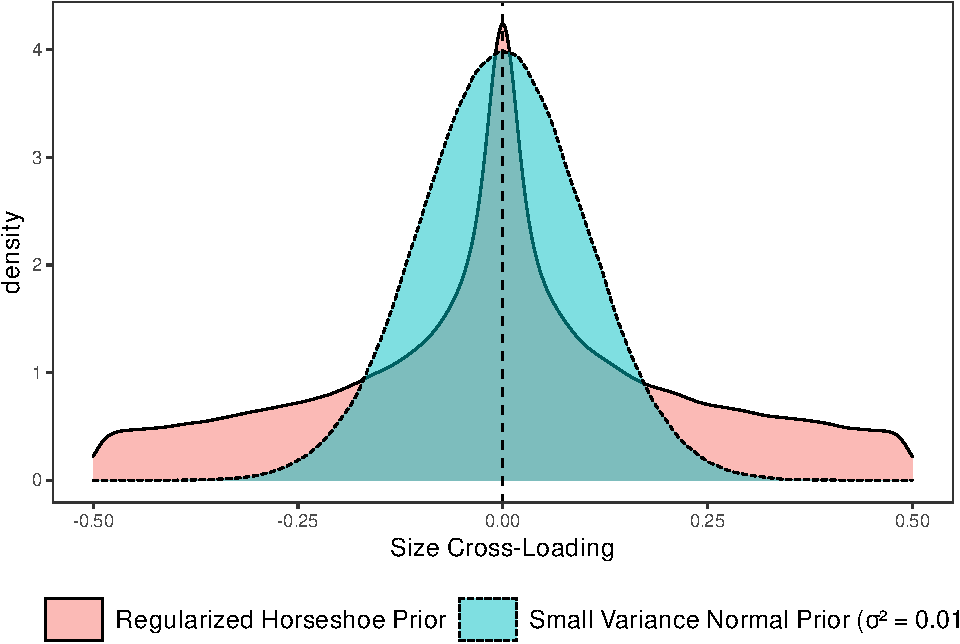
\includegraphics{JMBKoch_report_files/figure-latex/unnamed-chunk-1-1.pdf}
\caption{\label{fig:unnamed-chunk-1}Density Plots of the Regularization Priors of Interest}
\end{figure}

\hypertarget{the-current-study}{%
\section{The current study}\label{the-current-study}}

While the Regularized Horseshoe Prior has been shown to perform excellently in the selection of relevant predictors in regression (Piironen \& Vehtari, 2017b; Van Erp et al., 2019), no previous research has validated its performance in selecting relevant cross-loadings in CFA. To fill this gap, we aim to compare the RHSP to the SVNP in their performance in selecting the true factor structure in CFA. Below we present our preliminary results regarding the performance of the SVNP.

\hypertarget{study-procedure-and-parameters}{%
\subsection{Study Procedure and Parameters}\label{study-procedure-and-parameters}}

In order to assess the performance of the SVNP in regularizing cross-loadings in Bayesian Regularized SEM, a Monte Carlo simulation study was conducted using STAN (Stan Development Team, 2021). All code that was used to run the simulation study can be openly accessed on the author's \href{https://github.com/JMBKoch/1vs2StepBayesianRegSEM}{github}. The models were sampled using the No-U-Turn-Sampler (Homan \& Gelman, 2014), with two chains, a burnin-period of 2000 and a chain-length of 4000. These sampling parameters were identified in pilot-runs to be required for the RHSP to reach convergence, and were therefore also used for the SVNP in order to ensure a fair comparison.

\hypertarget{true-model-and-conditions}{%
\subsection{True Model and Conditions}\label{true-model-and-conditions}}

The datasets were simulated based on a true 2-factor model, with three items per factor, and a factor correlation of 0.5. The factors were scaled by fixing their means to zero and their variances to 1. All main-loadings were set to 0.75, and all residual variances to 0.3. We included two truly non-zero cross-loadings, that of factor 1 on item 4, and that of factor 2 on item 3. The true model is summarized below, both in equations (Appendix A) and graphically (Figure 1). We varied the magnitude of the two non-zero cross-loadings between 0.2 and 0.5. Next, we varied the sample sizes of the simulated datasets between 100 and 200. This choice was made because for simple factor models researchers would be unlikely to collect larger sample sizes in practice. Finally, based on the recommendations of Muthen and Asparouhov (2012), we included three levels of the hyper-parameter \(\sigma^2\): 0.001, 0.01, 0.1. This left us with a total number of 2 x 2 x 3 = 12 individual sets of conditions. Per set of conditions, 200 iterations were run, yielding a total of 2400 posterior samples.

\hypertarget{outcomes}{%
\subsection{Outcomes}\label{outcomes}}

As outcomes, we first considered the Mean (Absolute) Bias of all estimated model parameters (). Next, we also computed the Relative Bias and Mean Squared Error (MSE, Morris, White, \& Crowther, 2019). Next, we computed the power for the truly non-zero cross-loadings, i.e.~the probability of correctly identifying them as non-zero. For the truly zero cross-loadings we computed the Type-I Error Rate, hence the probability of wrongly selecting these cross-loadings as non-zero. For these last two outcomes, in order to select cross-loadings as zero, several selection rules were used based on recommendations Zhang, Pan, and Ip (2021). First, a number of thresholds were considered, where a cross-loading is selected to be zero when the absolute value of its posterior estimates falls below a certain value. Specifically we considered three thresholds: 0, 0.1, 0.15. Moreover, we selected cross-loadings based on whether or not their 95\%, 90\%, 80\%, and 50\% credible interval contained zero. Note that for all outcomes we computed two versions, one based on mean and one based on median posterior estimates. The latter is only reported in case of relevant deviations from the former.

\hypertarget{results}{%
\section{Results}\label{results}}

\hypertarget{convergence}{%
\subsection{Convergence}\label{convergence}}

In terms of convergence, the SVNP showed excellent performance. Across all iterations and configurations of conditions, there were not a single parameter for which \(\hat{R} < 1.05\). The lowest value of the Effective Sample Size \(N_{eff}\) was still a 39.4\% of the chain length, which is still a very acceptable proporation. For the largest majority of runs \(N_{eff}\) even exceeded 50\% of the chain length (96\% for the parameter with the largest percentage of \(\frac{N_{eff}}{N_{chain}} < 0.5\)). Moreover, across all runs there was not a single divergent transition. Therefore, none of the 2400 posterior samples had to be disregarded.

\hypertarget{main-results}{%
\subsection{Main Results}\label{main-results}}

The mean absolute bias of all model parameters is summarized below in Figure 3. The outcome is summarized for the different parameters as follows. For cross-loadings

\begin{figure}
\centering
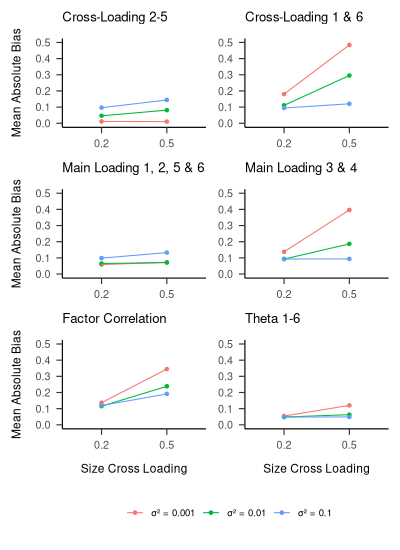
\includegraphics{~/1vs2StepBayesianRegSEM/Rmd/figures/allPars.png}
\caption{Main Results: Mean Absolute Bias in the Model Parameters.}
\end{figure}

\hypertarget{conclusions-and-discussion}{%
\section{Conclusions and Discussion}\label{conclusions-and-discussion}}

\clearpage

\hypertarget{references}{%
\section{References}\label{references}}

~

\begingroup
\setlength{\parindent}{-0.5in}
\setlength{\leftskip}{0.5in}

\hypertarget{refs}{}
\begin{CSLReferences}{1}{0}
\leavevmode\vadjust pre{\hypertarget{ref-bollen_structural_1989}{}}%
Bollen, K. A. (1989). \emph{Structural {Equations} with {Latent} {Variables}}. John Wiley \& Sons.

\leavevmode\vadjust pre{\hypertarget{ref-carvalho_horseshoe_2010}{}}%
Carvalho, C. M., Polson, N. G., \& Scott, J. G. (2010). The horseshoe estimator for sparse signals. \emph{Biometrika}, \emph{97}(2), 465--480. \url{https://doi.org/10.1093/biomet/asq017}

\leavevmode\vadjust pre{\hypertarget{ref-cox_principles_2006}{}}%
Cox, D. R. (2006). \emph{Principles of {Statistical} {Inference}}. Cambridge University Press.

\leavevmode\vadjust pre{\hypertarget{ref-ghosh_use_2018}{}}%
Ghosh, J., Li, Y., \& Mitra, R. (2018). On the {Use} of {Cauchy} {Prior} {Distributions} for {Bayesian} {Logistic} {Regression}. \emph{Bayesian Analysis}, \emph{13}(2), 359--383. \url{https://doi.org/10.1214/17-BA1051}

\leavevmode\vadjust pre{\hypertarget{ref-hastie_statistical_2015}{}}%
Hastie, T., Tibshirani, R., \& Wainwright, M. (2015). Statistical learning with sparsity. \emph{Monographs on Statistics and Applied Probability}, \emph{143}, 143.

\leavevmode\vadjust pre{\hypertarget{ref-hoerl_ridge_2000}{}}%
Hoerl, A. E., \& Kennard, R. W. (2000). Ridge {Regression}: {Biased} {Estimation} for {Nonorthogonal} {Problems}. \emph{Technometrics}, \emph{42}(1), 80--86. \url{https://doi.org/10.2307/1271436}

\leavevmode\vadjust pre{\hypertarget{ref-homan_no-u-turn_2014}{}}%
Homan, M. D., \& Gelman, A. (2014). The {No}-{U}-turn sampler: Adaptively setting path lengths in {Hamiltonian} {Monte} {Carlo}. \emph{The Journal of Machine Learning Research}, \emph{15}(1), 1593--1623.

\leavevmode\vadjust pre{\hypertarget{ref-hsiang_bayesian_1975}{}}%
Hsiang, T. C. (1975). A {Bayesian} {View} on {Ridge} {Regression}. \emph{Journal of the Royal Statistical Society. Series D (The Statistician)}, \emph{24}(4), 267--268. \url{https://doi.org/10.2307/2987923}

\leavevmode\vadjust pre{\hypertarget{ref-james_introduction_2021}{}}%
James, G., Witten, D., Hastie, T., \& Tibshirani, R. (2021). \emph{An {Introduction} to {Statistical} {Learning}: With {Applications} in {R}}. New York, NY: Springer US. \url{https://doi.org/10.1007/978-1-0716-1418-1}

\leavevmode\vadjust pre{\hypertarget{ref-lu_bayesian_2016}{}}%
Lu, Z.-H., Chow, S.-M., \& Loken, E. (2016). Bayesian {Factor} {Analysis} as a {Variable}-{Selection} {Problem}: {Alternative} {Priors} and {Consequences}. \emph{Multivariate Behavioral Research}, \emph{51}(4), 519--539. \url{https://doi.org/10.1080/00273171.2016.1168279}

\leavevmode\vadjust pre{\hypertarget{ref-maccallum_model_1992}{}}%
MacCallum, R. C., Roznowski, M., \& Necowitz, L. B. (1992). Model modifications in covariance structure analysis: The problem of capitalization on chance. \emph{Psychological Bulletin}, \emph{111}(3), 490--504. \url{https://doi.org/10.1037/0033-2909.111.3.490}

\leavevmode\vadjust pre{\hypertarget{ref-morris_using_2019}{}}%
Morris, T. P., White, I. R., \& Crowther, M. J. (2019). Using simulation studies to evaluate statistical methods. \emph{Statistics in Medicine}, \emph{38}(11), 2074--2102. \url{https://doi.org/10.1002/sim.8086}

\leavevmode\vadjust pre{\hypertarget{ref-muthen_bayesian_2012}{}}%
Muthen, B., \& Asparouhov, T. (2012). Bayesian {SEM}: {A} more flexible representation of substantive theory, 78. \url{https://doi.org/10.1037/a0026802}

\leavevmode\vadjust pre{\hypertarget{ref-park_bayesian_2008}{}}%
Park, T., \& Casella, G. (2008). The {Bayesian} {Lasso}. \emph{Journal of the American Statistical Association}, \emph{103}(482), 681--686. \url{https://doi.org/10.1198/016214508000000337}

\leavevmode\vadjust pre{\hypertarget{ref-piironen_hyperprior_2017}{}}%
Piironen, J., \& Vehtari, A. (2017a). On the {Hyperprior} {Choice} for the {Global} {Shrinkage} {Parameter} in the {Horseshoe} {Prior}. In \emph{Proceedings of the 20th {International} {Conference} on {Artificial} {Intelligence} and {Statistics}} (pp. 905--913). PMLR. Retrieved from \url{https://proceedings.mlr.press/v54/piironen17a.html}

\leavevmode\vadjust pre{\hypertarget{ref-piironen_sparsity_2017}{}}%
Piironen, J., \& Vehtari, A. (2017b). Sparsity information and regularization in the horseshoe and other shrinkage priors. \emph{Electronic Journal of Statistics}, \emph{11}(2), 5018--5051. \url{https://doi.org/10.1214/17-EJS1337SI}

\leavevmode\vadjust pre{\hypertarget{ref-stan_development_team_stan_2021}{}}%
Stan Development Team. (2021). Stan {User} {Guide}. Retrieved from \url{https://mc-stan.org/docs/2_27/stan-users-guide-2_27.pdf}

\leavevmode\vadjust pre{\hypertarget{ref-tibshirani_regression_1996}{}}%
Tibshirani, R. (1996). Regression {Shrinkage} and {Selection} {Via} the {Lasso}. \emph{Journal of the Royal Statistical Society: Series B (Methodological)}, \emph{58}(1), 267--288. \url{https://doi.org/10.1111/j.2517-6161.1996.tb02080.x}

\leavevmode\vadjust pre{\hypertarget{ref-van_erp_shrinkage_2019}{}}%
Van Erp, S., Oberski, D. L., \& Mulder, J. (2019). Shrinkage priors for {Bayesian} penalized regression. \emph{Journal of Mathematical Psychology}, \emph{89}, 31--50. \url{https://doi.org/10.1016/j.jmp.2018.12.004}

\leavevmode\vadjust pre{\hypertarget{ref-zhang_criteria_2021}{}}%
Zhang, L., Pan, J., \& Ip, E. H. (2021). Criteria for {Parameter} {Identification} in {Bayesian} {Lasso} {Methods} for {Covariance} {Analysis}: {Comparing} {Rules} for {Thresholding}, \emph{p} -value, and {Credible} {Interval}. \emph{Structural Equation Modeling: A Multidisciplinary Journal}, 1--10. \url{https://doi.org/10.1080/10705511.2021.1945456}

\end{CSLReferences}

\endgroup

\clearpage

\begingroup
\setlength{\parskip}{0in}
\setlength{\parindent}{-0.27in}
\setlength{\leftskip}{0.5in}

\hypertarget{appendix}{%
\section{Appendix}\label{appendix}}

\hypertarget{appendix-a-true-model}{%
\subsection{Appendix A: True Model}\label{appendix-a-true-model}}

For every individual i in i = 1,\ldots,N:
\[Y_i \sim \mathcal{N}(\mathbf{0}, \Sigma),\] where
\[\Sigma = \Lambda\Psi\Lambda',\]
\[\Lambda = 
    \begin{bmatrix}
    0.75 & 0 \\
    0.75 & 0 \\
    0.75 & 0.2/0.5 \\
    0.2/0.5 & 0.75 \\
    0 & 0.75 \\
    0 & 0.75
    \end{bmatrix},\]
\[\Psi =
    \begin{bmatrix}
     1 & 0.5 \\
     0.5 & 1
    \end{bmatrix}
,\] and
\[\Theta = diag[0.3, 0.3, 0.3, 0.3, 0.3, 0.3].\]

\hypertarget{figures}{%
\section{Figures}\label{figures}}


\end{document}
